\section{Research Direction}

\begin{frame}{Challenges and Opportunities}
    \begin{enumerate}
        \item The majority of existing LLMs are closed-sourced, such as OpenAI's GPT-4, or have an infeasibly large number of parameters for training within the scope of this research, such as the 70-billion parameter LLaMa model.

        \item The source code of common data science libraries like Pandas and Numpy is extensive, posing a challenge for LLMs to sufficiently capture the context of the full codebase.

        \item Although complex, software systems have structured and well-tested code, allowing the feedback from critic models to be reliable.
    \end{enumerate}
\end{frame}

\begin{frame}{Research Direction}
    \begin{figure}[!htb]
        \centering
        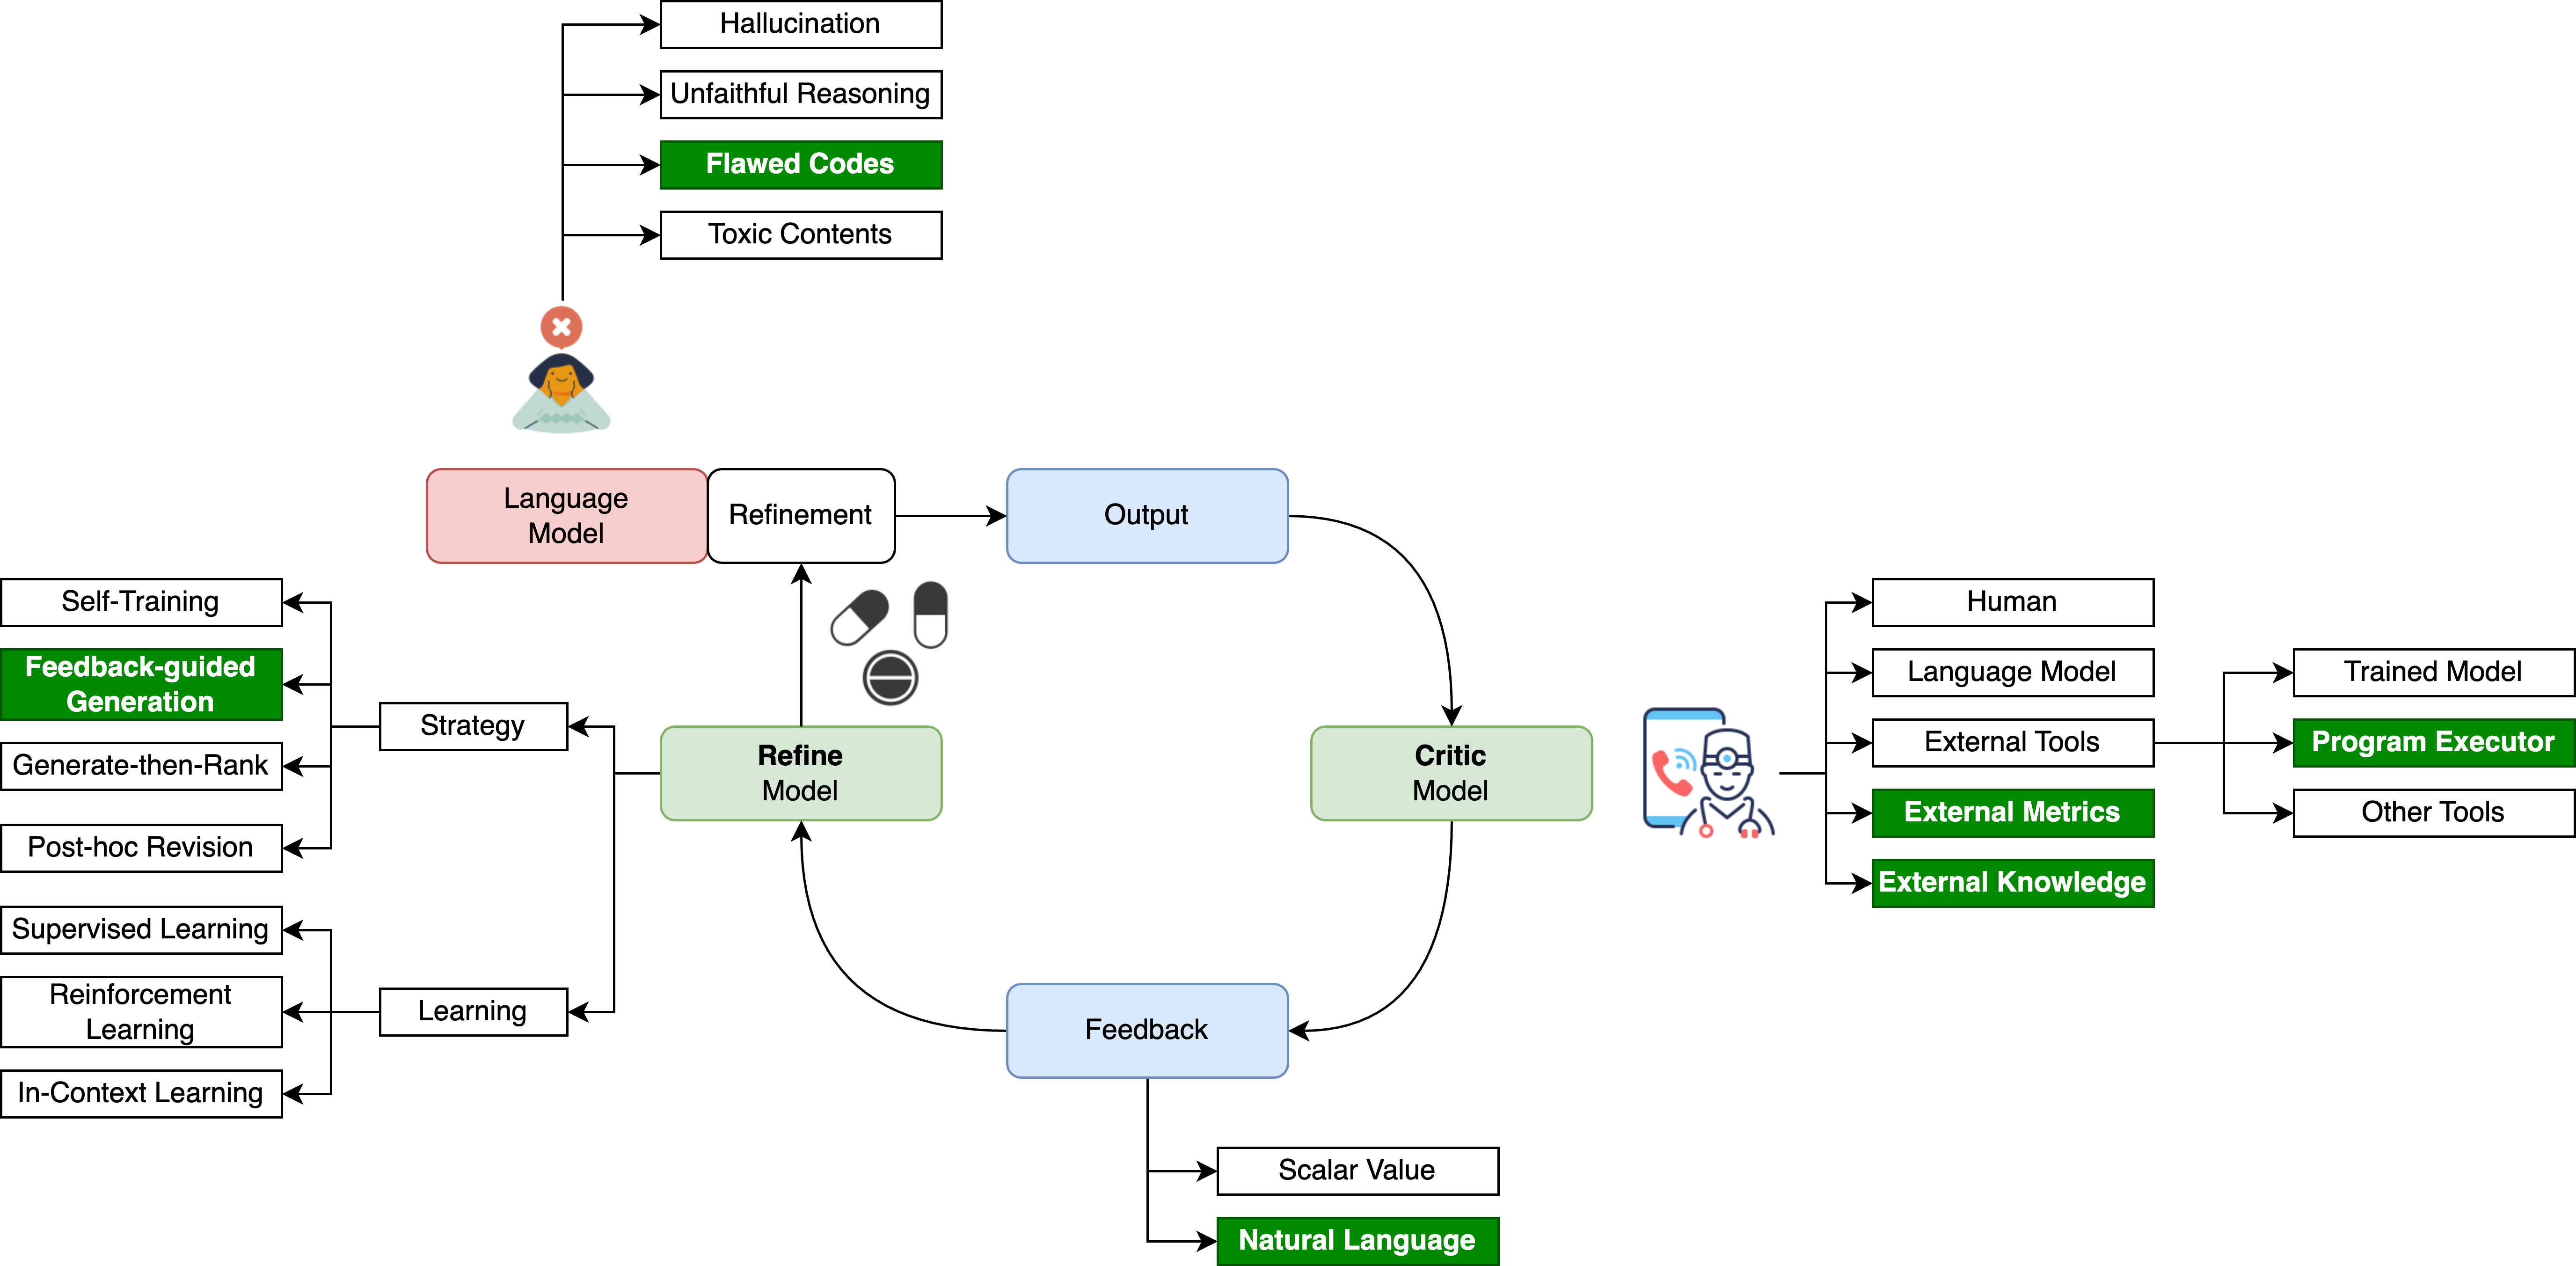
\includegraphics[scale=0.045]{img/direction_of_research}
        \captionsetup{font=small}
        \caption{Research Direction.}
    \end{figure}
    This research will improve flawed code generation by LLMs using feedback from unit tests (\textbf{External Metrics}), tracebacks (\textbf{Program Executor}) and source code analysis (\textbf{External Knowledge}) via \textbf{Feedback-Guided Generation}.
\end{frame}
